\documentclass[aspectratio=169]{beamer}

% ── Tema base ─────────────────────────────────────────────────────────────────
\usetheme{default}
\usecolortheme{default}
\setbeamertemplate{navigation symbols}{}

% ── Colores UTEC ──────────────────────────────────────────────────────────────
\definecolor{utecblue}{RGB}{0,82,155}
\definecolor{uteccyan}{RGB}{0,174,219}
\definecolor{lightgray}{RGB}{245,245,245}

\setbeamercolor{frametitle}{bg=utecblue, fg=white}
\setbeamerfont{frametitle}{size=\large, series=\bfseries}

\setbeamercolor{title}{fg=white}
\setbeamercolor{subtitle}{fg=uteccyan}
\setbeamercolor{author}{fg=white}
\setbeamercolor{institute}{fg=white!80}
\setbeamercolor{date}{fg=white!70}

\setbeamercolor{block title}{bg=utecblue, fg=white}
\setbeamercolor{block body}{bg=utecblue!8, fg=black}
\setbeamercolor{alertblock title}{bg=uteccyan!80!black, fg=white}
\setbeamercolor{alertblock body}{bg=uteccyan!12, fg=black}

\setbeamercolor{itemize item}{fg=utecblue}
\setbeamercolor{itemize subitem}{fg=uteccyan}
\setbeamertemplate{itemize item}{\small$\blacktriangleright$}
\setbeamertemplate{itemize subitem}{\small$\triangleright$}

\setbeamertemplate{footline}{%
  \hfill\usebeamerfont{footline}\insertframenumber\,/\,\inserttotalframenumber\hspace{1em}\vspace{0.4em}
}

\setbeamercolor{background canvas}{bg=white}

% ── Paquetes ──────────────────────────────────────────────────────────────────
\usepackage[utf8]{inputenc}
\usepackage[T1]{fontenc}
\usepackage{graphicx}
\usepackage{booktabs}
\usepackage{amsmath}
\usepackage{amssymb}
\usepackage{tikz}
\usepackage{array}
\usepackage{colortbl}
\usepackage{pgfplots}
\usepackage{xcolor}
\usepackage{url}
\pgfplotsset{compat=1.18}
\usetikzlibrary{arrows.meta, shapes.geometric, positioning, fit, backgrounds}

% ── Comando para placeholder de imagen/video ──────────────────────────────────
\newcommand{\imgplaceholder}[2][8cm]{%
  \begin{tikzpicture}
    \node[draw=utecblue!40, dashed, fill=utecblue!5,
          minimum width=#1, minimum height=4cm,
          font=\small\color{utecblue!70}, align=center,
          rounded corners=4pt] {#2};
  \end{tikzpicture}%
}

% ── Metadatos ─────────────────────────────────────────────────────────────────
\title{Multi-Object Tracking in UAV Imagery}
\subtitle{Method 1 (Baseline): YOLOv11 + SORT}
\author{Rensso Victor Hugo Mora Colque}
\institute{Computer Vision --- UTEC}
\date{2026-I}

% =============================================================================
\begin{document}
% =============================================================================

% ── SLIDE 1: PORTADA ──────────────────────────────────────────────────────────
{
\setbeamercolor{background canvas}{bg=white}
\begin{frame}[plain]
  \vspace{1.2cm}
  \centering
  {\color{utecblue}\Large\bfseries Method 1 (Baseline): YOLOv11 + SORT\par}
  \vspace{0.4em}
  \color{utecblue!50}\rule{0.5\textwidth}{0.4pt}\par
  \vspace{0.8em}
  {\color{utecblue!80}\small Computer Vision --- UTEC\par}
  {\color{utecblue!80}\small PC4: Detection and Tracking\par}
  \vspace{0.4em}
  {\color{utecblue!70}\small Rensso Victor Hugo Mora Colque\par}
  {\color{utecblue!60}\small 2026-I\par}
\end{frame}
}


% ── SLIDE 2: YOLO VISIÓN GENERAL ──────────────────────────────────────────────
\begin{frame}{YOLOv11 Architecture}
  \centering
  \vspace{0.2cm}
  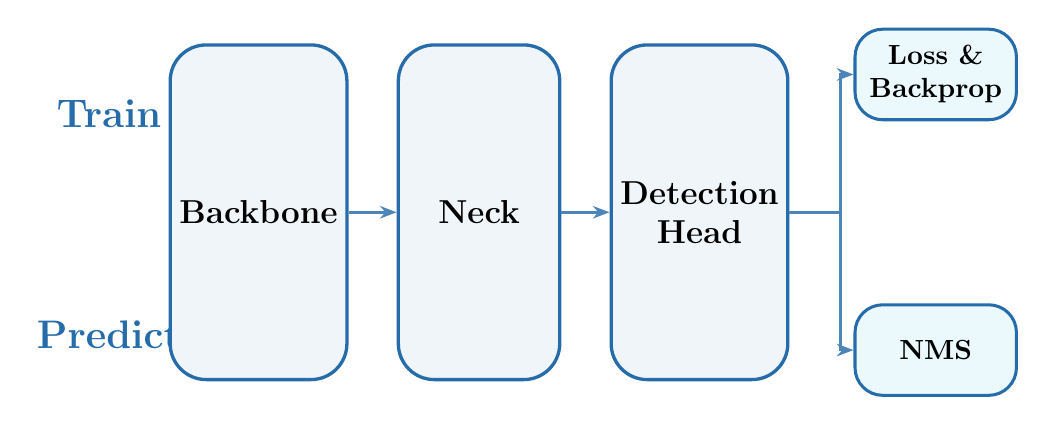
\begin{tikzpicture}[
      module/.style={
          draw=utecblue!85,
          fill=utecblue!6,
          rounded corners=13pt,
          line width=1.2pt,
          minimum width=2.05cm,
          minimum height=4.25cm,
          font=\large\bfseries,
          align=center
        },
      sidebox/.style={
          draw=utecblue!85,
          fill=uteccyan!8,
          rounded corners=10pt,
          line width=1.1pt,
          minimum width=2.05cm,
          minimum height=1.15cm,
          font=\normalsize\bfseries,
          align=center
        },
      flow/.style={-{Stealth[length=6pt]}, utecblue!70, line width=1.0pt},
      label/.style={font=\Large\bfseries, text=utecblue!85}
    ]
    \node[label] (train) at (-5.65, 1.25) {Train};
    \node[label] (predict) at (-5.65,-1.55) {Predict};

    \node[module] (backbone) at (-3.75,0) {Backbone};
    \node[module] (neck) at (-0.95,0) {Neck};
    \node[module] (head) at (1.85,0) {Detection\\Head};

    \node[sidebox] (loss) at (4.85,1.75) {Loss \&\\Backprop};
    \node[sidebox] (nms) at (4.85,-1.75) {NMS};

    \draw[flow] (backbone) -- (neck);
    \draw[flow] (neck) -- (head);
    \draw[utecblue!70, line width=1.0pt] (head.east) -- ++(0.65,0) coordinate (split);
    \draw[flow] (split) |- (loss.west);
    \draw[flow] (split) |- (nms.west);
  \end{tikzpicture}
\end{frame}


% ── SLIDE 3: CBS Block ──────────────────────────────────────────────
\begin{frame}{YOLOv11: Conv + BatchNorm + SiLU Block}
  \centering
  \begin{columns}[c]
    \begin{column}{0.39\textwidth}
      \centering
      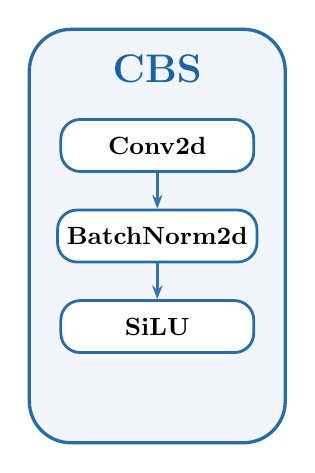
\begin{tikzpicture}[
          cbsbox/.style={
              draw=utecblue!85,
              fill=utecblue!5,
              rounded corners=15pt,
              line width=1.2pt,
              minimum width=3.25cm,
              minimum height=5.25cm
            },
          layer/.style={
              draw=utecblue!85,
              fill=white,
              rounded corners=7pt,
              line width=1.0pt,
              minimum width=2.45cm,
              minimum height=0.66cm,
              font=\small\bfseries,
              align=center
            },
          arr/.style={-{Stealth[length=5pt]}, utecblue!80, line width=1.0pt}
        ]
        \node[cbsbox] (outer) at (0,0) {};
        \node[font=\Large\bfseries, text=utecblue!90] at (0,2.12) {CBS};
        \node[layer] (conv) at (0,1.15) {Conv2d};
        \node[layer] (bn) at (0,0.0) {BatchNorm2d};
        \node[layer] (silu) at (0,-1.15) {SiLU};
        \draw[arr] (conv) -- (bn);
        \draw[arr] (bn) -- (silu);
      \end{tikzpicture}
    \end{column}
    \begin{column}{0.57\textwidth}
      \centering
      \[
        \mathrm{SiLU}(x)=x\cdot\frac{1}{1+e^{-x}}
      \]
      \vspace{0.2cm}
      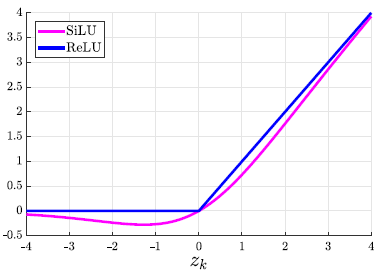
\includegraphics[width=0.9\linewidth]{figures/silu.png}
    \end{column}
  \end{columns}
\end{frame}


% ── SLIDE 4: Bottle Neck ──────────────────────────────────────────────
\begin{frame}{YOLOv11: Bottle Neck Block}
  \begin{columns}[c]
    \begin{column}{0.40\textwidth}
      \centering
      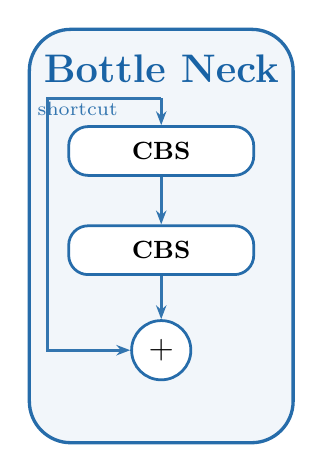
\begin{tikzpicture}[
          outer/.style={
              draw=utecblue!85,
              fill=utecblue!5,
              rounded corners=15pt,
              line width=1.2pt,
              minimum width=3.35cm,
              minimum height=5.25cm
            },
          layer/.style={
              draw=utecblue!85,
              fill=white,
              rounded corners=7pt,
              line width=1.0pt,
              minimum width=2.35cm,
              minimum height=0.62cm,
              font=\small\bfseries,
              align=center
            },
          sum/.style={
              circle,
              draw=utecblue!85,
              fill=white,
              line width=1.0pt,
              minimum size=0.62cm,
              font=\large\bfseries
            },
          arr/.style={-{Stealth[length=5pt]}, utecblue!80, line width=1.0pt},
          shortcut/.style={-{Stealth[length=5pt]}, utecblue!80, line width=1.1pt}
        ]
        \node[outer] at (0,0) {};
        \node[font=\Large\bfseries, text=utecblue!90] at (0,2.13) {Bottle Neck};

        \node[layer] (cbs1) at (0,1.08) {CBS};
        \node[layer] (cbs2) at (0,-0.18) {CBS};
        \node[sum] (add) at (0,-1.45) {$+$};

        \coordinate (input) at (0,1.75);
        \draw[arr] (input) -- (cbs1.north);
        \draw[arr] (cbs1) -- (cbs2);
        \draw[arr] (cbs2) -- (add);

        \draw[shortcut] (input) -- ++(-1.45,0) |- (add.west);
        \node[font=\scriptsize, text=utecblue!80] at (-1.06,1.62) {shortcut};
      \end{tikzpicture}
    \end{column}
    \begin{column}{0.56\textwidth}
      \textbf{Bottleneck idea}
      \begin{itemize}
        \item Two CBS layers transform the feature map with low extra cost.
        \item The shortcut adds the input back to the output:
      \end{itemize}
      \[
        \mathbf{y} = F(\mathbf{x}) + \mathbf{x}
      \]
      \begin{itemize}
        \item Same residual principle as a ResNet block: preserve useful input information and improve gradient flow.
        \item CBS means \textbf{Conv + BatchNorm + SiLU}; convolution extracts features, BatchNorm stabilizes training, and SiLU adds nonlinearity.
      \end{itemize}
    \end{column}
  \end{columns}
\end{frame}


% ── SLIDE 5: C3K2 ──────────────────────────────────────────────
\begin{frame}{YOLOv11: C3K2 Block}
  \begin{columns}[T]
    \begin{column}{0.45\textwidth}
      \textbf{C3K block}
      \begin{itemize}
        \item Repeats bottleneck blocks $n$ times to deepen feature extraction.
        \item Final concat keeps both transformed and preserved features.
      \end{itemize}
      \vspace{0.2em}
      \textbf{C3K2 improvement}
      \begin{itemize}
        \item Replaces each repeated bottleneck with a smaller C3K unit.
        \item Keeps multi-stage feature reuse while reducing cost.
      \end{itemize}
    \end{column}
    \begin{column}{0.55\textwidth}
      \centering
      \vspace{1cm}
      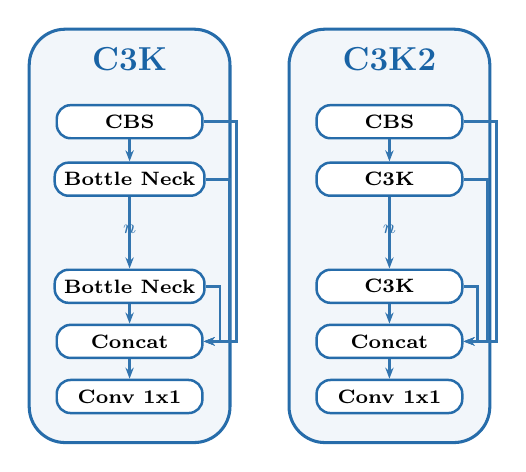
\begin{tikzpicture}[
          outer/.style={
              draw=utecblue!85,
              fill=utecblue!5,
              rounded corners=13pt,
              line width=1.1pt,
              minimum width=2.55cm,
              minimum height=5.25cm
            },
          layer/.style={
              draw=utecblue!85,
              fill=white,
              rounded corners=5pt,
              line width=0.9pt,
              minimum width=1.85cm,
              minimum height=0.42cm,
              font=\scriptsize\bfseries,
              align=center
            },
          arr/.style={-{Stealth[length=4pt]}, utecblue!80, line width=0.9pt},
          shortcut/.style={-{Stealth[length=4pt]}, utecblue!80, line width=1.0pt}
        ]
        \node[outer] (c3kbox) at (-1.65,0) {};
        \node[font=\large\bfseries, text=utecblue!90] at (-1.65,2.25) {C3K};
        \node[layer] (c3k_cbs) at (-1.65,1.45) {CBS};
        \node[layer] (c3k_bn1) at (-1.65,0.72) {Bottle Neck};
        \node[font=\scriptsize, text=utecblue!80] at (-1.65,0.08) {$n$};
        \node[layer] (c3k_bn2) at (-1.65,-0.64) {Bottle Neck};
        \node[layer] (c3k_concat) at (-1.65,-1.34) {Concat};
        \node[layer] (c3k_conv) at (-1.65,-2.04) {Conv 1x1};

        \draw[arr] (c3k_cbs) -- (c3k_bn1);
        \draw[arr] (c3k_bn1) -- (c3k_bn2);
        \draw[arr] (c3k_bn2) -- (c3k_concat);
        \draw[arr] (c3k_concat) -- (c3k_conv);
        \draw[shortcut] (c3k_cbs.east) -- ++(0.42,0) |- (c3k_concat.east);
        \draw[shortcut] (c3k_bn1.east) -- ++(0.30,0) |- (c3k_concat.east);
        \draw[shortcut] (c3k_bn2.east) -- ++(0.18,0) |- (c3k_concat.east);

        \node[outer] (c3k2box) at (1.65,0) {};
        \node[font=\large\bfseries, text=utecblue!90] at (1.65,2.25) {C3K2};
        \node[layer] (c3k2_cbs) at (1.65,1.45) {CBS};
        \node[layer] (c3k2_c3k1) at (1.65,0.72) {C3K};
        \node[font=\scriptsize, text=utecblue!80] at (1.65,0.08) {$n$};
        \node[layer] (c3k2_c3k2) at (1.65,-0.64) {C3K};
        \node[layer] (c3k2_concat) at (1.65,-1.34) {Concat};
        \node[layer] (c3k2_conv) at (1.65,-2.04) {Conv 1x1};

        \draw[arr] (c3k2_cbs) -- (c3k2_c3k1);
        \draw[arr] (c3k2_c3k1) -- (c3k2_c3k2);
        \draw[arr] (c3k2_c3k2) -- (c3k2_concat);
        \draw[arr] (c3k2_concat) -- (c3k2_conv);
        \draw[shortcut] (c3k2_cbs.east) -- ++(0.42,0) |- (c3k2_concat.east);
        \draw[shortcut] (c3k2_c3k1.east) -- ++(0.30,0) |- (c3k2_concat.east);
        \draw[shortcut] (c3k2_c3k2.east) -- ++(0.18,0) |- (c3k2_concat.east);
      \end{tikzpicture}
    \end{column}
  \end{columns}
\end{frame}


% ── SLIDE 6: Backbone ──────────────────────────────────────────────
\begin{frame}{YOLOv11: Backbone Step}
  \begin{columns}[c]
    \begin{column}{0.5\textwidth}
      \centering
      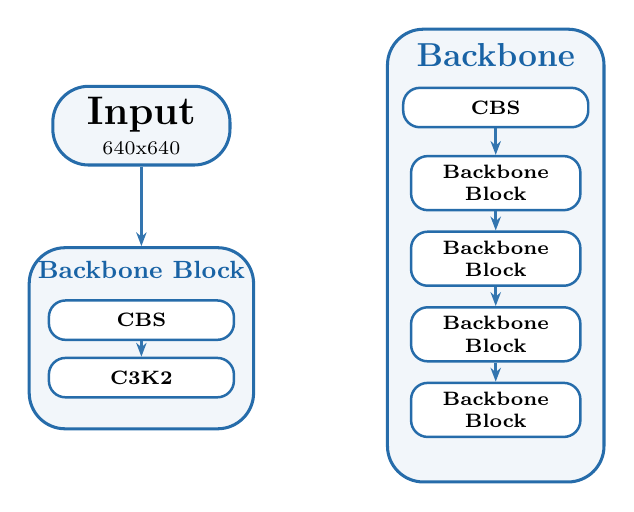
\begin{tikzpicture}[
          outer/.style={
              draw=utecblue!85,
              fill=utecblue!5,
              rounded corners=13pt,
              line width=1.1pt,
              align=center
            },
          smallbox/.style={
              draw=utecblue!85,
              fill=white,
              rounded corners=6pt,
              line width=0.9pt,
              minimum width=2.35cm,
              minimum height=0.50cm,
              font=\scriptsize\bfseries,
              align=center
            },
          blockbox/.style={
              draw=utecblue!85,
              fill=white,
              rounded corners=6pt,
              line width=0.9pt,
              minimum width=2.15cm,
              minimum height=0.56cm,
              font=\scriptsize\bfseries,
              align=center
            },
          arr/.style={-{Stealth[length=5pt]}, utecblue!80, line width=1.0pt}
        ]
        \node[outer, minimum width=2.25cm, minimum height=1.0cm] (input) at (-3.35,1.65)
        {\Large\bfseries Input\\[-1pt]\scriptsize 640x640};

        \node[outer, minimum width=2.85cm, minimum height=2.30cm] (bb) at (-3.35,-1.05) {};
        \node[font=\small\bfseries, text=utecblue!90] at (-3.35,-0.18) {Backbone Block};
        \node[smallbox] (bb_cbs) at (-3.35,-0.82) {CBS};
        \node[smallbox] (bb_c3k2) at (-3.35,-1.55) {C3K2};

        \draw[arr] (input.south) -- ++(0,-0.75) -- (bb.north);
        \draw[arr] (bb_cbs) -- (bb_c3k2);

        \node[outer, minimum width=2.75cm, minimum height=5.75cm] (backbone) at (1.15,0) {};
        \node[font=\large\bfseries, text=utecblue!90] at (1.15,2.55) {Backbone};
        \node[smallbox] (b_cbs) at (1.15,1.88) {CBS};
        \node[blockbox] (b1) at (1.15,0.92) {Backbone\\Block};
        \node[blockbox] (b2) at (1.15,-0.04) {Backbone\\Block};
        \node[blockbox] (b3) at (1.15,-1.00) {Backbone\\Block};
        \node[blockbox] (b4) at (1.15,-1.96) {Backbone\\Block};

        \draw[arr] (b_cbs) -- (b1);
        \draw[arr] (b1) -- (b2);
        \draw[arr] (b2) -- (b3);
        \draw[arr] (b3) -- (b4);
      \end{tikzpicture}
    \end{column}
    \begin{column}{0.5\textwidth}
      \textbf{Backbone role}
      \begin{itemize}
        \item Receives the input image and extracts visual features at increasing depth.
        \item Early CBS layer detects simple patterns such as edges, colors, and small textures.
        \item Each stage reduces spatial resolution and increases semantic information for detection.
        \item Output feature maps feed the neck
      \end{itemize}
    \end{column}
  \end{columns}
\end{frame}


% ── SLIDE 7: SPFF ──────────────────────────────────────────────
\begin{frame}{YOLOv11: Spatial Pyramid Pooling Fast}
  \begin{columns}[c]
    \begin{column}{0.46\textwidth}
      \begin{itemize}
        \item It expands the receptive field before features are passed to the neck.
        \item Repeated max-pooling captures context at several spatial scales.
        \item Concat merges local and pooled features so the neck can fuse richer multi-scale information.
        \item It is efficient because sequential pooling reuses intermediate outputs instead of computing separate large kernels.
      \end{itemize}
    \end{column}
    \begin{column}{0.50\textwidth}
      \centering
      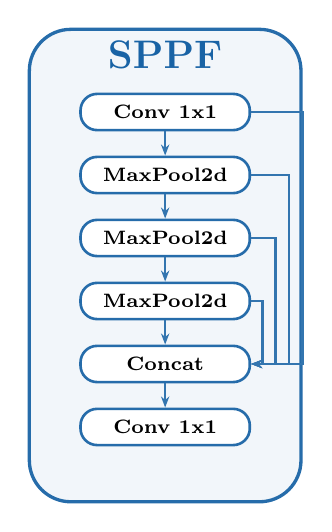
\begin{tikzpicture}[
          outer/.style={
              draw=utecblue!85,
              fill=utecblue!5,
              rounded corners=15pt,
              line width=1.2pt,
              minimum width=3.45cm,
              minimum height=6.00cm
            },
          layer/.style={
              draw=utecblue!85,
              fill=white,
              rounded corners=6pt,
              line width=0.95pt,
              minimum width=2.15cm,
              minimum height=0.46cm,
              font=\scriptsize\bfseries,
              align=center
            },
          arr/.style={-{Stealth[length=4pt]}, utecblue!80, line width=0.9pt},
          skip/.style={-{Stealth[length=4pt]}, utecblue!80, line width=1.0pt}
        ]
        \node[outer] at (0,0) {};
        \node[font=\Large\bfseries, text=utecblue!90] at (0,2.68) {SPPF};

        \node[layer] (conv1) at (0,1.95) {Conv 1x1};
        \node[layer] (pool1) at (0,1.15) {MaxPool2d};
        \node[layer] (pool2) at (0,0.35) {MaxPool2d};
        \node[layer] (pool3) at (0,-0.45) {MaxPool2d};
        \node[layer] (concat) at (0,-1.25) {Concat};
        \node[layer] (conv2) at (0,-2.05) {Conv 1x1};

        \draw[arr] (conv1) -- (pool1);
        \draw[arr] (pool1) -- (pool2);
        \draw[arr] (pool2) -- (pool3);
        \draw[arr] (pool3) -- (concat);
        \draw[arr] (concat) -- (conv2);

        \draw[skip] (conv1.east) -- ++(0.65,0) |- (concat.east);
        \draw[skip] (pool1.east) -- ++(0.48,0) |- (concat.east);
        \draw[skip] (pool2.east) -- ++(0.31,0) |- (concat.east);
        \draw[skip] (pool3.east) -- ++(0.14,0) |- (concat.east);
      \end{tikzpicture}
    \end{column}
  \end{columns}
\end{frame}


% ── SLIDE 8: C2PSA ──────────────────────────────────────────────
\begin{frame}{YOLOv11: Cross Stage Partial Self-Attention}
  \begin{columns}[T]
    \begin{column}{0.5\textwidth}
      \centering
      \vspace{-0.15cm}
      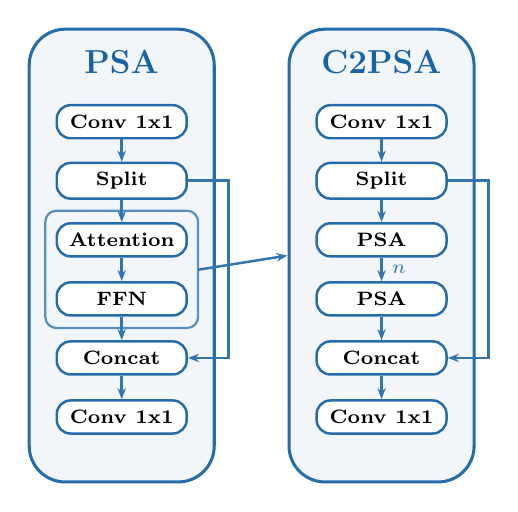
\begin{tikzpicture}[
          outer/.style={
              draw=utecblue!85,
              fill=utecblue!5,
              rounded corners=13pt,
              line width=1.1pt,
              minimum width=2.35cm,
              minimum height=5.75cm
            },
          layer/.style={
              draw=utecblue!85,
              fill=white,
              rounded corners=5pt,
              line width=0.9pt,
              minimum width=1.65cm,
              minimum height=0.42cm,
              font=\scriptsize\bfseries,
              align=center
            },
          arr/.style={-{Stealth[length=4pt]}, utecblue!80, line width=0.9pt},
          skip/.style={-{Stealth[length=4pt]}, utecblue!80, line width=1.0pt}
        ]
        \node[outer] (psa_box) at (-1.65,0) {};
        \node[font=\large\bfseries, text=utecblue!90] at (-1.65,2.46) {PSA};
        \node[layer] (p_conv1) at (-1.65,1.70) {Conv 1x1};
        \node[layer] (p_split) at (-1.65,0.95) {Split};
        \node[layer] (attn) at (-1.65,0.20) {Attention};
        \node[layer] (ffn) at (-1.65,-0.55) {FFN};
        \node[layer] (p_concat) at (-1.65,-1.30) {Concat};
        \node[layer] (p_conv2) at (-1.65,-2.05) {Conv 1x1};
        \draw[utecblue!65, rounded corners=4pt, line width=0.8pt] (-2.62,0.57) rectangle (-0.68,-0.92);
        \coordinate (psa_core_east) at (-0.68,-0.18);

        \draw[arr] (p_conv1) -- (p_split);
        \draw[arr] (p_split) -- (attn);
        \draw[arr] (attn) -- (ffn);
        \draw[arr] (ffn) -- (p_concat);
        \draw[arr] (p_concat) -- (p_conv2);
        \draw[skip] (p_split.east) -- ++(0.52,0) |- (p_concat.east);

        \node[outer] (c2_box) at (1.65,0) {};
        \node[font=\large\bfseries, text=utecblue!90] at (1.65,2.46) {C2PSA};
        \node[layer] (c_conv1) at (1.65,1.70) {Conv 1x1};
        \node[layer] (split) at (1.65,0.95) {Split};
        \node[layer] (psa1) at (1.65,0.20) {PSA};
        \node[layer] (psa2) at (1.65,-0.55) {PSA};
        \node[layer] (c_concat) at (1.65,-1.30) {Concat};
        \node[layer] (c_conv2) at (1.65,-2.05) {Conv 1x1};

        \draw[arr] (c_conv1) -- (split);
        \draw[arr] (split) -- (psa1);
        \draw[arr] (psa1) -- node[midway, right, font=\scriptsize\bfseries] {$n$} (psa2);
        \draw[arr] (psa2) -- (c_concat);
        \draw[arr] (c_concat) -- (c_conv2);
        \draw[skip] (split.east) -- ++(0.52,0) |- (c_concat.east);

        \draw[arr] (psa_core_east) -- (c2_box.west);
      \end{tikzpicture}
    \end{column}
    \begin{column}{0.5\textwidth}
      \small
      \textbf{Attention core}
      \[
        \mathrm{Attn}(Q,K,V)=
        \mathrm{softmax}\!\left(
        \frac{QK^\top}{\sqrt{d_k}}
        \right)V
      \]
      \begin{itemize}
        \item $QK^\top$ scores how strongly each position should attend to other positions.
        \item $\sqrt{d_k}$ stabilizes score scale before softmax.
        \item PSA adds global spatial context, then FFN refines channel features.
        \item C2PSA first splits channels, applies PSA on one path, then concatenates and compresses with Conv $1{\times}1$.
      \end{itemize}
    \end{column}
  \end{columns}
\end{frame}


% ── SLIDE 9: Neck ──────────────────────────────────────────────
\begin{frame}{YOLOv11: Neck Step}
  \centering
  \vspace{-0.15cm}
  \resizebox{\textwidth}{!}{%
    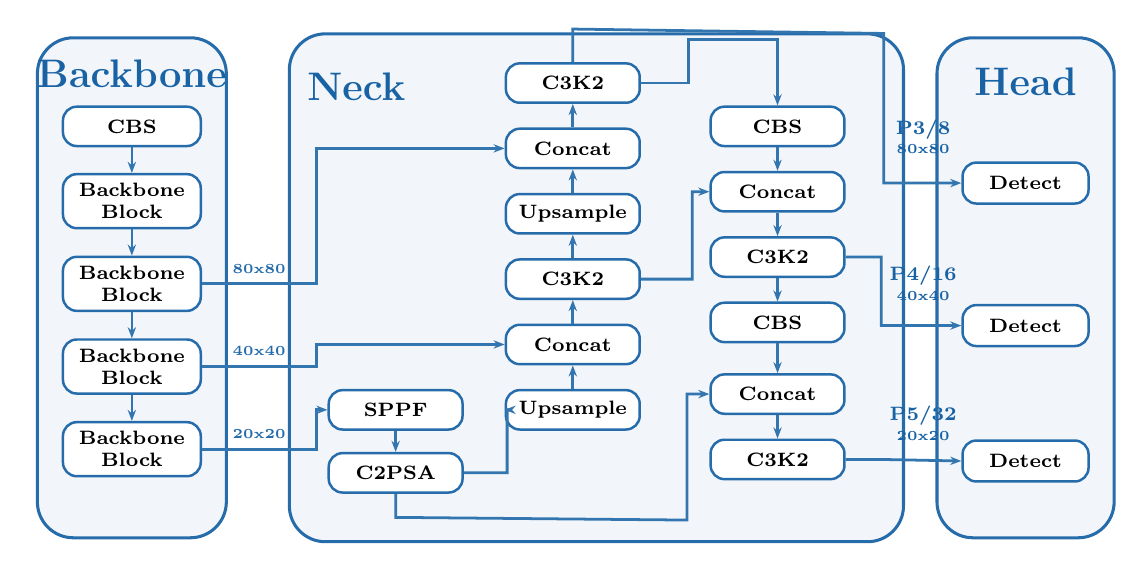
\begin{tikzpicture}[
        outer/.style={
            draw=utecblue!85,
            fill=utecblue!5,
            rounded corners=13pt,
            line width=1.1pt
          },
        block/.style={
            draw=utecblue!85,
            fill=white,
            rounded corners=5pt,
            line width=0.9pt,
            minimum width=1.75cm,
            minimum height=0.50cm,
            font=\scriptsize\bfseries,
            align=center
          },
        neckblock/.style={
            draw=utecblue!85,
            fill=white,
            rounded corners=5pt,
            line width=0.9pt,
            minimum width=1.70cm,
            minimum height=0.50cm,
            font=\scriptsize\bfseries,
            align=center
          },
        detect/.style={
            draw=utecblue!85,
            fill=white,
            rounded corners=5pt,
            line width=0.9pt,
            minimum width=1.60cm,
            minimum height=0.52cm,
            font=\scriptsize\bfseries,
            align=center
          },
        arr/.style={-{Stealth[length=4pt]}, utecblue!80, line width=0.95pt},
        route/.style={-{Stealth[length=4pt]}, utecblue!80, line width=1.0pt}
      ]
      \node[outer, minimum width=2.40cm, minimum height=6.35cm] (backbone_box) at (-5.90,0) {};
      \node[font=\Large\bfseries, text=utecblue!90] at (-5.90,2.72) {Backbone};
      \node[block] (bb_cbs) at (-5.90,2.05) {CBS};
      \node[block] (bb1) at (-5.90,1.10) {Backbone\\Block};
      \node[block] (bb2) at (-5.90,0.05) {Backbone\\Block};
      \node[block] (bb3) at (-5.90,-1.00) {Backbone\\Block};
      \node[block] (bb4) at (-5.90,-2.05) {Backbone\\Block};

      \draw[arr] (bb_cbs) -- (bb1);
      \draw[arr] (bb1) -- (bb2);
      \draw[arr] (bb2) -- (bb3);
      \draw[arr] (bb3) -- (bb4);

      \node[outer, minimum width=7.80cm, minimum height=6.45cm] (neck_box) at (0.00,0) {};
      \node[font=\Large\bfseries, text=utecblue!90] at (-3.05,2.55) {Neck};

      \node[neckblock] (sppf) at (-2.55,-1.55) {SPPF};
      \node[neckblock] (c2psa) at (-2.55,-2.35) {C2PSA};

      \node[neckblock] (up1) at (-0.30,-1.55) {Upsample};
      \node[neckblock] (concat1) at (-0.30,-0.72) {Concat};
      \node[neckblock] (c3k2_1) at (-0.30,0.11) {C3K2};
      \node[neckblock] (up2) at (-0.30,0.94) {Upsample};
      \node[neckblock] (concat2) at (-0.30,1.77) {Concat};
      \node[neckblock] (c3k2_2) at (-0.30,2.60) {C3K2};

      \node[neckblock] (r_cbs1) at (2.30,2.05) {CBS};
      \node[neckblock] (r_concat1) at (2.30,1.22) {Concat};
      \node[neckblock] (r_c3k2_1) at (2.30,0.39) {C3K2};
      \node[neckblock] (r_cbs2) at (2.30,-0.44) {CBS};
      \node[neckblock] (r_concat2) at (2.30,-1.35) {Concat};
      \node[neckblock] (r_c3k2_2) at (2.30,-2.18) {C3K2};

      \node[outer, minimum width=2.25cm, minimum height=6.35cm] (head_box) at (5.45,0) {};
      \node[font=\Large\bfseries, text=utecblue!90] at (5.45,2.62) {Head};
      \node[detect] (d3) at (5.45,1.33) {Detect};
      \node[detect] (d4) at (5.45,-0.48) {Detect};
      \node[detect] (d5) at (5.45,-2.20) {Detect};

      \draw[arr] (sppf) -- (c2psa);
      \draw[route] (c2psa.east) -- ++(0.55,0) -- ++(0,0.80) -- (up1.west);
      \draw[arr] (up1) -- (concat1);
      \draw[arr] (concat1) -- (c3k2_1);
      \draw[arr] (c3k2_1) -- (up2);
      \draw[arr] (up2) -- (concat2);
      \draw[arr] (concat2) -- (c3k2_2);

      \draw[route] (c3k2_2.east) -- ++(0.60,0) -- ++(0,0.55) -| (r_cbs1.north);
      \draw[arr] (r_cbs1) -- (r_concat1);
      \draw[arr] (r_concat1) -- (r_c3k2_1);
      \draw[arr] (r_c3k2_1) -- (r_cbs2);
      \draw[arr] (r_cbs2) -- (r_concat2);
      \draw[arr] (r_concat2) -- (r_c3k2_2);

      \draw[route] (bb2.east) -- node[above,font=\tiny\bfseries,text=utecblue!85] {80x80} ++(1.45,0) |- (concat2.west);
      \draw[route] (bb3.east) -- node[above,font=\tiny\bfseries,text=utecblue!85] {40x40} ++(1.45,0) |- (concat1.west);
      \draw[route] (bb4.east) -- node[above,font=\tiny\bfseries,text=utecblue!85] {20x20} ++(1.45,0) |- (sppf.west);

      \draw[route] (c2psa.south) -- ++(0,-0.30) -- (1.15,-2.95) -- (1.15,-1.35) -- (r_concat2.west);
      \draw[route] (c3k2_1.east) -- ++(0.65,0) -- ++(0,1.11) -- (r_concat1.west);

      \node[font=\scriptsize\bfseries, text=utecblue!90, align=center] at (4.15,1.92) {P3/8\\[-1pt]\tiny 80x80};
      \node[font=\scriptsize\bfseries, text=utecblue!90, align=center] at (4.15,0.06) {P4/16\\[-1pt]\tiny 40x40};
      \node[font=\scriptsize\bfseries, text=utecblue!90, align=center] at (4.15,-1.72) {P5/32\\[-1pt]\tiny 20x20};

      \draw[route] (c3k2_2.north) -- ++(0,0.42) -- (3.65,3.23) -- (3.65,1.33) -- (d3.west);
      \draw[route] (r_c3k2_1.east) -- ++(0.45,0) -- ++(0,-0.87) -- (d4.west);
      \draw[route] (r_c3k2_2.east) -- ++(0.45,0) -- (d5.west);
    \end{tikzpicture}%
  }
\end{frame}


% ── SLIDE 10: Detection Head Block ──────────────────────────────────────────────
\begin{frame}{YOLOv11: Detection Head Step}
  \centering
  \vspace{-0.15cm}
  \resizebox{0.98\textwidth}{!}{%
    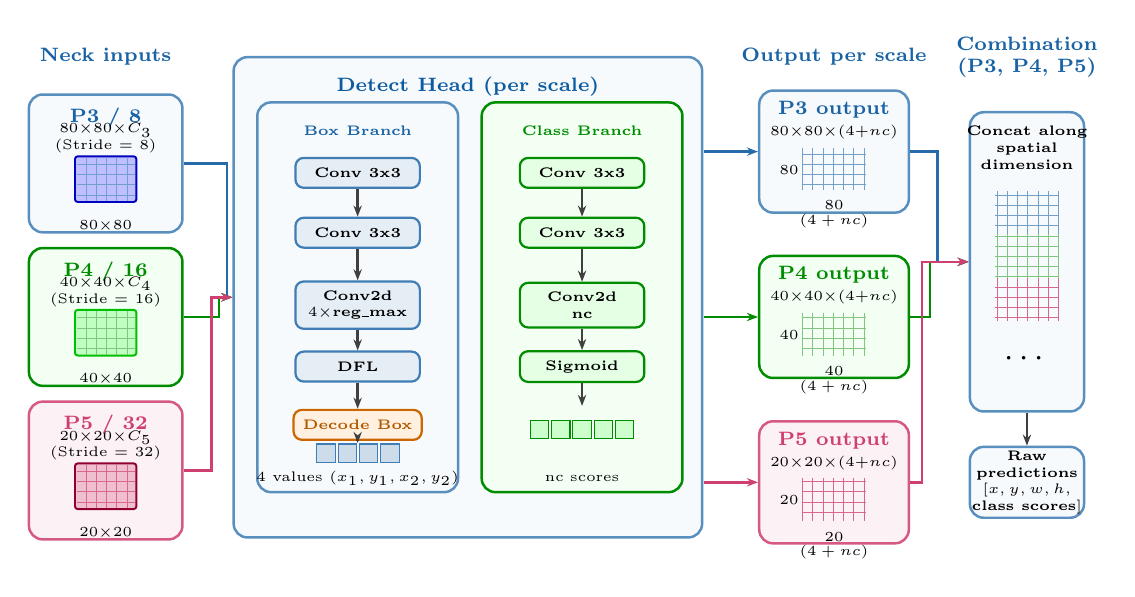
\begin{tikzpicture}[
        panel/.style={
            draw=utecblue!65,
            fill=utecblue!3,
            rounded corners=5pt,
            line width=0.9pt,
            align=center
          },
        greenpanel/.style={
            draw=green!55!black,
            fill=green!5,
            rounded corners=5pt,
            line width=0.9pt,
            align=center
          },
        purplepanel/.style={
            draw=purple!65,
            fill=purple!5,
            rounded corners=5pt,
            line width=0.9pt,
            align=center
          },
        layerblue/.style={
            draw=utecblue!75,
            fill=utecblue!10,
            rounded corners=3pt,
            line width=0.8pt,
            minimum width=1.58cm,
            minimum height=0.38cm,
            font=\tiny\bfseries,
            align=center
          },
        decodebox/.style={
            draw=orange!80!black,
            fill=orange!12,
            rounded corners=3pt,
            line width=0.8pt,
            minimum width=1.58cm,
            minimum height=0.38cm,
            font=\tiny\bfseries,
            text=orange!70!black,
            align=center
          },
        layergreen/.style={
            draw=green!55!black,
            fill=green!10,
            rounded corners=3pt,
            line width=0.8pt,
            minimum width=1.58cm,
            minimum height=0.38cm,
            font=\tiny\bfseries,
            align=center
          },
        cubeblue/.style={
            draw=blue!75!black,
            fill=blue!25,
            rounded corners=1pt,
            line width=0.7pt,
            minimum width=0.78cm,
            minimum height=0.58cm
          },
        cubegreen/.style={
            draw=green!75!black,
            fill=green!25,
            rounded corners=1pt,
            line width=0.7pt,
            minimum width=0.78cm,
            minimum height=0.58cm
          },
        cubepurple/.style={
            draw=purple!75!black,
            fill=purple!25,
            rounded corners=1pt,
            line width=0.7pt,
            minimum width=0.78cm,
            minimum height=0.58cm
          },
        arrblue/.style={-{Stealth[length=4pt]}, utecblue!85, line width=0.9pt},
        arrgreen/.style={-{Stealth[length=4pt]}, green!55!black, line width=0.9pt},
        arrpurple/.style={-{Stealth[length=4pt]}, purple!75, line width=0.9pt},
        arr/.style={-{Stealth[length=4pt]}, black!75, line width=0.85pt}
      ]
      % Inputs
      \node[font=\scriptsize\bfseries, text=utecblue!90] at (-6.25,3.05) {Neck inputs};

      \node[panel, minimum width=1.95cm, minimum height=1.75cm] (p3in) at (-6.25,1.70) {};
      \node[font=\scriptsize\bfseries, text=utecblue!90] at (-6.25,2.28) {P3 / 8};
      \node[font=\tiny, align=center] at (-6.25,2.02) {$80{\times}80{\times}C_3$\\(Stride = 8)};
      \node[cubeblue] at (-6.25,1.50) {};
      \draw[step=0.13cm, utecblue!55, line width=0.25pt] (-6.62,1.22) grid (-5.88,1.78);
      \node[font=\tiny] at (-6.25,0.91) {$80{\times}80$};

      \node[greenpanel, minimum width=1.95cm, minimum height=1.75cm] (p4in) at (-6.25,-0.25) {};
      \node[font=\scriptsize\bfseries, text=green!55!black] at (-6.25,0.33) {P4 / 16};
      \node[font=\tiny, align=center] at (-6.25,0.07) {$40{\times}40{\times}C_4$\\(Stride = 16)};
      \node[cubegreen] at (-6.25,-0.45) {};
      \draw[step=0.13cm, green!55!black!50, line width=0.25pt] (-6.62,-0.73) grid (-5.88,-0.17);
      \node[font=\tiny] at (-6.25,-1.04) {$40{\times}40$};

      \node[purplepanel, minimum width=1.95cm, minimum height=1.75cm] (p5in) at (-6.25,-2.20) {};
      \node[font=\scriptsize\bfseries, text=purple!75] at (-6.25,-1.62) {P5 / 32};
      \node[font=\tiny, align=center] at (-6.25,-1.88) {$20{\times}20{\times}C_5$\\(Stride = 32)};
      \node[cubepurple] at (-6.25,-2.40) {};
      \draw[step=0.13cm, purple!60, line width=0.25pt] (-6.62,-2.68) grid (-5.88,-2.12);
      \node[font=\tiny] at (-6.25,-2.99) {$20{\times}20$};

      % Central detect head
      \node[panel, minimum width=5.95cm, minimum height=6.10cm] (head) at (-1.65,0) {};
      \node[font=\scriptsize\bfseries, text=utecblue!95] at (-1.65,2.68) {Detect Head (per scale)};

      \node[panel, minimum width=2.55cm, minimum height=4.95cm] (boxbranch) at (-3.05,0.00) {};
      \node[font=\tiny\bfseries, text=utecblue!90] at (-3.05,2.12) {Box Branch};
      \node[layerblue] (bconv1) at (-3.05,1.58) {Conv 3x3};
      \node[layerblue] (bconv2) at (-3.05,0.82) {Conv 3x3};
      \node[layerblue, minimum height=0.50cm] (bbox) at (-3.05,-0.10) {Conv2d\\$4{\times}$reg\_max};
      \node[layerblue] (dfl) at (-3.05,-0.88) {DFL};
      \node[decodebox] (decode) at (-3.05,-1.62) {Decode Box};
      \node[font=\tiny] at (-3.05,-2.30) {4 values $(x_1,y_1,x_2,y_2)$};
      \foreach \x in {-3.45,-3.18,-2.91,-2.64}
      \node[draw=utecblue!75, fill=utecblue!20, minimum width=0.19cm, minimum height=0.19cm] at (\x,-1.98) {};

      \node[greenpanel, minimum width=2.55cm, minimum height=4.95cm] (classbranch) at (-0.20,0.00) {};
      \node[font=\tiny\bfseries, text=green!55!black] at (-0.20,2.12) {Class Branch};
      \node[layergreen] (cconv1) at (-0.20,1.58) {Conv 3x3};
      \node[layergreen] (cconv2) at (-0.20,0.82) {Conv 3x3};
      \node[layergreen, minimum height=0.50cm] (cls) at (-0.20,-0.10) {Conv2d\\nc};
      \node[layergreen] (sig) at (-0.20,-0.88) {Sigmoid};
      \node[font=\tiny] at (-0.20,-2.30) {nc scores};
      \foreach \x in {-0.74,-0.47,-0.20,0.07,0.34}
      \node[draw=green!55!black, fill=green!20, minimum width=0.19cm, minimum height=0.19cm] at (\x,-1.68) {};

      \draw[arr] (bconv1) -- (bconv2);
      \draw[arr] (bconv2) -- (bbox);
      \draw[arr] (bbox) -- (dfl);
      \draw[arr] (dfl) -- (decode);
      \draw[arr] (decode) -- ++(0,-0.23);
      \draw[arr] (cconv1) -- (cconv2);
      \draw[arr] (cconv2) -- (cls);
      \draw[arr] (cls) -- (sig);
      \draw[arr] (sig) -- ++(0,-0.50);

      \draw[arrblue] (p3in.east) -- ++(0.55,0) |- (head.west);
      \draw[arrgreen] (p4in.east) -- ++(0.45,0) |- (head.west);
      \draw[arrpurple] (p5in.east) -- ++(0.35,0) |- (head.west);

      % Outputs by scale
      \node[font=\scriptsize\bfseries, text=utecblue!90] at (3.00,3.05) {Output per scale};

      \node[panel, minimum width=1.90cm, minimum height=1.55cm] (p3out) at (3.00,1.85) {};
      \node[font=\scriptsize\bfseries, text=utecblue!90] at (3.00,2.38) {P3 output};
      \node[font=\tiny, align=center] at (3.00,2.10) {$80{\times}80{\times}(4{+}nc)$};
      \draw[step=0.13cm, utecblue!55, line width=0.25pt] (2.60,1.36) grid (3.40,1.90);
      \node[font=\tiny] at (2.43,1.62) {80};
      \node[font=\tiny] at (3.00,1.17) {80};
      \node[font=\tiny] at (3.00,0.97) {$(4+nc)$};

      \node[greenpanel, minimum width=1.90cm, minimum height=1.55cm] (p4out) at (3.00,-0.25) {};
      \node[font=\scriptsize\bfseries, text=green!55!black] at (3.00,0.28) {P4 output};
      \node[font=\tiny, align=center] at (3.00,0.00) {$40{\times}40{\times}(4{+}nc)$};
      \draw[step=0.13cm, green!55!black!50, line width=0.25pt] (2.60,-0.74) grid (3.40,-0.20);
      \node[font=\tiny] at (2.43,-0.48) {40};
      \node[font=\tiny] at (3.00,-0.94) {40};
      \node[font=\tiny] at (3.00,-1.14) {$(4+nc)$};

      \node[purplepanel, minimum width=1.90cm, minimum height=1.55cm] (p5out) at (3.00,-2.35) {};
      \node[font=\scriptsize\bfseries, text=purple!75] at (3.00,-1.82) {P5 output};
      \node[font=\tiny, align=center] at (3.00,-2.10) {$20{\times}20{\times}(4{+}nc)$};
      \draw[step=0.13cm, purple!60, line width=0.25pt] (2.60,-2.84) grid (3.40,-2.30);
      \node[font=\tiny] at (2.43,-2.58) {20};
      \node[font=\tiny] at (3.00,-3.04) {20};
      \node[font=\tiny] at (3.00,-3.24) {$(4+nc)$};

      \draw[arrblue] (1.35,1.85) -- (p3out.west);
      \draw[arrgreen] (1.35,-0.25) -- (p4out.west);
      \draw[arrpurple] (1.35,-2.35) -- (p5out.west);

      % Combination
      \node[font=\scriptsize\bfseries, text=utecblue!90, align=center] at (5.45,3.05)
      {Combination\\(P3, P4, P5)};
      \node[panel, minimum width=1.45cm, minimum height=3.80cm] (combo) at (5.45,0.45) {};
      \node[font=\tiny\bfseries, align=center] at (5.45,1.90) {Concat along\\spatial\\dimension};
      \draw[step=0.13cm, utecblue!55, line width=0.25pt] (5.05,0.80) grid (5.85,1.35);
      \draw[step=0.13cm, green!55!black!50, line width=0.25pt] (5.05,0.25) grid (5.85,0.80);
      \draw[step=0.13cm, purple!60, line width=0.25pt] (5.05,-0.30) grid (5.85,0.25);
      \node[font=\large\bfseries] at (5.45,-0.78) {$\cdots$};

      \node[panel, minimum width=1.45cm, minimum height=0.90cm] (pred) at (5.45,-2.35) {};
      \node[font=\tiny\bfseries, align=center] at (5.45,-2.35)
      {Raw\\predictions\\$[x,y,w,h,$\\class scores$]$};

      \draw[arrblue] (p3out.east) -- ++(0.35,0) |- (combo.west);
      \draw[arrgreen] (p4out.east) -- ++(0.25,0) |- (combo.west);
      \draw[arrpurple] (p5out.east) -- ++(0.15,0) |- (combo.west);
      \draw[arr] (combo.south) -- (pred.north);
    \end{tikzpicture}%
  }
\end{frame}


% ── SLIDE 11: DFL + Decode Box ──────────────────────────────────────────────
\begin{frame}{YOLOv11: Distribution Focal Loss and Decode Box}
  \centering
  \vspace{-0.15cm}
  \resizebox{\textwidth}{!}{%
    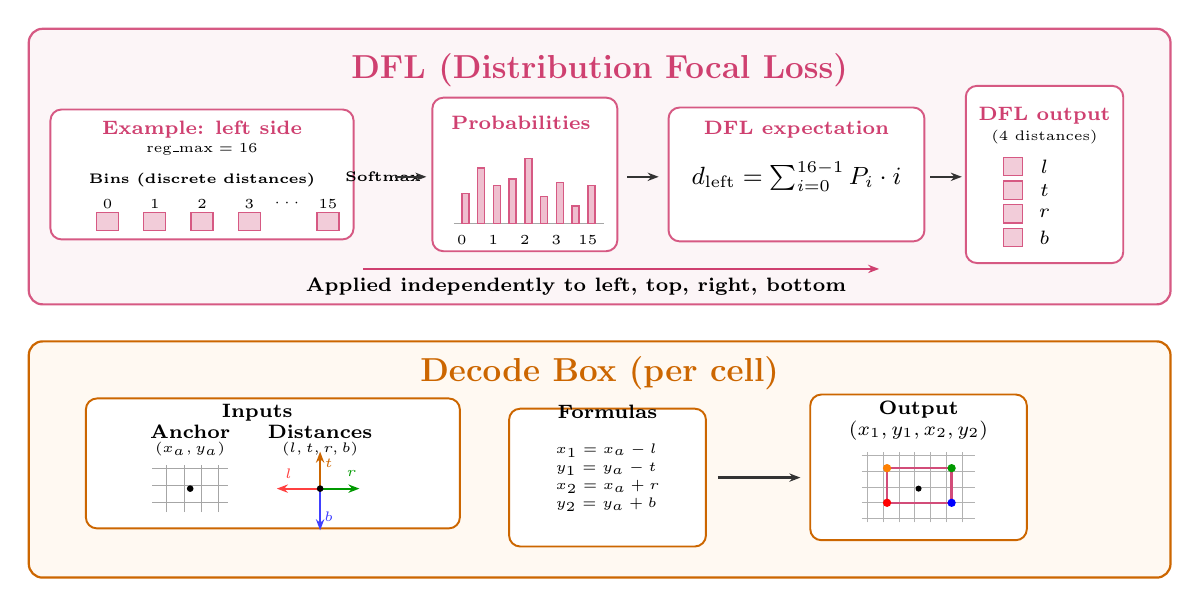
\begin{tikzpicture}[
        panel/.style={
            draw=purple!65,
            fill=purple!4,
            rounded corners=5pt,
            line width=0.8pt
          },
        orangepanel/.style={
            draw=orange!80!black,
            fill=orange!5,
            rounded corners=5pt,
            line width=0.8pt
          },
        box/.style={
            draw=purple!65,
            fill=white,
            rounded corners=4pt,
            line width=0.7pt,
            minimum height=0.62cm,
            font=\scriptsize,
            align=center
          },
        orangebox/.style={
            draw=orange!80!black,
            fill=white,
            rounded corners=4pt,
            line width=0.7pt,
            minimum height=0.62cm,
            font=\scriptsize,
            align=center
          },
        arr/.style={-{Stealth[length=4pt]}, black!80, line width=0.8pt},
        parr/.style={-{Stealth[length=4pt]}, purple!75, line width=0.8pt},
        oarr/.style={-{Stealth[length=4pt]}, orange!80!black, line width=0.8pt}
      ]
      % DFL panel
      \node[panel, minimum width=14.5cm, minimum height=3.5cm] at (0,1.65) {};
      \node[font=\large\bfseries, text=purple!75] at (0,2.88) {DFL (Distribution Focal Loss)};

      \node[box, minimum width=3.85cm, minimum height=1.65cm] (bins) at (-5.05,1.55) {};
      \node[font=\scriptsize\bfseries, text=purple!75] at (-5.05,2.12) {Example: left side};
      \node[font=\tiny] at (-5.05,1.87) {$\mathrm{reg\_max}=16$};
      \node[font=\tiny\bfseries] at (-5.05,1.48) {Bins (discrete distances)};
      \node[font=\tiny] at (-6.25,1.18) {0};
      \node[font=\tiny] at (-5.65,1.18) {1};
      \node[font=\tiny] at (-5.05,1.18) {2};
      \node[font=\tiny] at (-4.45,1.18) {3};
      \node[font=\tiny] at (-3.95,1.18) {$\cdots$};
      \node[font=\tiny] at (-3.45,1.18) {15};
      \foreach \x in {-6.25,-5.65,-5.05,-4.45,-3.45}
      \node[draw=purple!65, fill=purple!20, minimum width=0.28cm, minimum height=0.22cm] at (\x,0.95) {};

      \node[font=\tiny\bfseries] at (-2.75,1.52) {Softmax};
      \draw[arr] (-2.60,1.52) -- (-2.20,1.52);

      \node[box, minimum width=2.35cm, minimum height=1.95cm] (prob) at (-0.95,1.55) {};
      \node[font=\scriptsize\bfseries, text=purple!75] at (-1,2.2) {Probabilities};
      \draw[black!35, line width=0.3pt] (-1.85,0.93) -- (0.05,0.93);
      \foreach \x/\h in {
          -1.75/0.38,
          -1.55/0.70,
          -1.35/0.48,
          -1.15/0.56,
          -0.95/0.82,
          -0.75/0.34,
          -0.55/0.52,
          -0.35/0.22,
          -0.15/0.48
        }
      \draw[purple!65, fill=purple!25, line width=0.5pt] (\x,0.93) rectangle ++(0.09,\h);
      \node[font=\tiny] at (-1.75,0.72) {0};
      \node[font=\tiny] at (-1.35,0.72) {1};
      \node[font=\tiny] at (-0.95,0.72) {2};
      \node[font=\tiny] at (-0.55,0.72) {3};
      \node[font=\tiny] at (-0.15,0.72) {15};

      \draw[arr] (0.35,1.52) -- (0.75,1.52);

      \node[box, minimum width=3.25cm, minimum height=1.70cm] (expect) at (2.50,1.55) {};
      \node[font=\scriptsize\bfseries, text=purple!75] at (2.50,2.12) {DFL expectation};
      \node[font=\small] at (2.50,1.52) {$d_{\mathrm{left}}=\sum_{i=0}^{16-1}P_i\cdot i$};

      \draw[arr] (4.2,1.52) -- (4.6,1.52);

      \node[box, minimum width=2cm, minimum height=2.25cm] (dflout) at (5.65,1.55) {};
      \node[font=\scriptsize\bfseries, text=purple!75] at (5.65,2.3) {DFL output};
      \node[font=\tiny] at (5.65,2.02) {(4 distances)};
      \node[font=\scriptsize\bfseries] at (5.65,1.65) {$l$};
      \node[font=\scriptsize\bfseries] at (5.65,1.35) {$t$};
      \node[font=\scriptsize\bfseries] at (5.65,1.05) {$r$};
      \node[font=\scriptsize\bfseries] at (5.65,0.75) {$b$};
      \foreach \y in {
          1.65,
          1.35,
          1.05,
          0.75
        }
      \node[draw=purple!65, fill=purple!20, minimum width=0.18cm, minimum height=0.18cm] at (5.25,\y) {};

      \draw[parr] (-3,0.35) -- (3.55,0.35);
      \node[font=\scriptsize\bfseries] at (-0.30,0.12) {Applied independently to left, top, right, bottom};

      % Decode panel
      \begin{scope}[yshift=-0.42cm]
        \node[orangepanel, minimum width=14.5cm, minimum height=3cm] at (0,-1.65) {};
        \node[font=\large\bfseries, text=orange!80!black] at (0,-0.55) {Decode Box (per cell)};

        \node[orangebox, minimum width=4.75cm, minimum height=1.65cm] (inputs) at (-4.15,-1.70) {};
        \node[font=\scriptsize\bfseries] at (-4.35,-1.05) {Inputs};
        \node[font=\scriptsize\bfseries] at (-5.20,-1.30) {Anchor};
        \node[font=\tiny] at (-5.20,-1.52) {$(x_a,y_a)$};
        \draw[step=0.22cm, black!35, line width=0.25pt] (-5.68,-2.32) grid (-4.72,-1.72);
        \fill[black] (-5.20,-2.02) circle (1.2pt);
        \node[font=\scriptsize\bfseries] at (-3.55,-1.30) {Distances};
        \node[font=\tiny] at (-3.55,-1.52) {$(l,t,r,b)$};
        \draw[oarr] (-3.55,-2.02) -- (-3.55,-1.55);
        \draw[red!75, -{Stealth[length=4pt]}, line width=0.8pt] (-3.55,-2.02) -- (-4.10,-2.02);
        \draw[green!60!black, -{Stealth[length=4pt]}, line width=0.8pt] (-3.55,-2.02) -- (-3.05,-2.02);
        \draw[blue!75, -{Stealth[length=4pt]}, line width=0.8pt] (-3.55,-2.02) -- (-3.55,-2.55);
        \fill[black] (-3.55,-2.02) circle (1.2pt);
        \node[font=\tiny, text=orange!80!black] at (-3.44,-1.70) {$t$};
        \node[font=\tiny, text=red!75] at (-3.95,-1.83) {$l$};
        \node[font=\tiny, text=green!60!black] at (-3.15,-1.83) {$r$};
        \node[font=\tiny, text=blue!75] at (-3.44,-2.38) {$b$};

        \node[orangebox, minimum width=2.50cm, minimum height=1.75cm] at (0.10,-1.88) {};
        \node[font=\scriptsize\bfseries] at (0.10,-1.05) {Formulas};
        \node[font=\tiny, align=left] at (0.10,-1.88)
        {$x_1=x_a-l$\\[0.08em]$y_1=y_a-t$\\[0.08em]$x_2=x_a+r$\\[0.08em]$y_2=y_a+b$};
        \draw[arr] (1.50,-1.88) -- (2.55,-1.88);

        \node[orangebox, minimum width=2.75cm, minimum height=1.85cm] (outbox) at (4.05,-1.75) {};
        \node[font=\scriptsize\bfseries] at (4.05,-1.02) {Output};
        \node[font=\scriptsize\bfseries] at (4.05,-1.28) {$(x_1,y_1,x_2,y_2)$};
        \draw[step=0.20cm, black!30, line width=0.25pt] (3.33,-2.45) grid (4.77,-1.55);
        \draw[purple!70, line width=0.9pt] (3.65,-2.20) rectangle (4.47,-1.76);
        \fill[orange] (3.65,-1.76) circle (1.5pt);
        \fill[green!60!black] (4.47,-1.76) circle (1.5pt);
        \fill[red] (3.65,-2.20) circle (1.5pt);
        \fill[blue] (4.47,-2.20) circle (1.5pt);
        \fill[black] (4.05,-2.02) circle (1.1pt);
      \end{scope}
    \end{tikzpicture}%
  }
\end{frame}


% ── SLIDE 12: Postprocesing and NMS ──────────────────────────────────────────────────
\begin{frame}{YOLOv11: Postprocessing and NMS}
  \centering
  \vspace{-0.15cm}
  \resizebox{\textwidth}{!}{%
    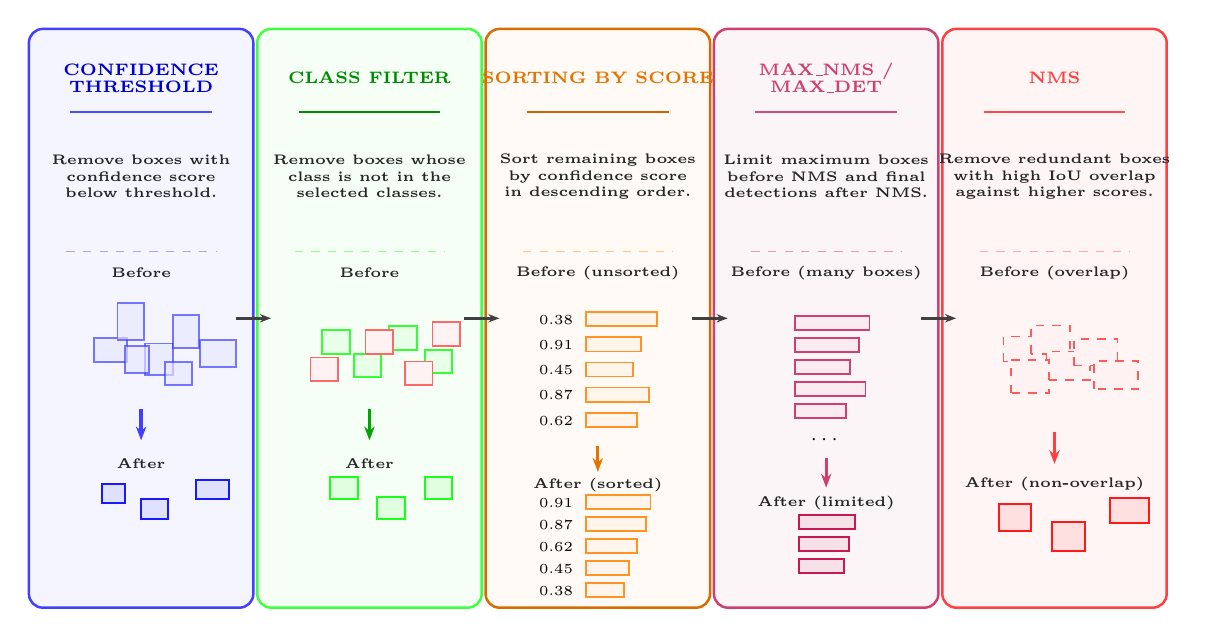
\begin{tikzpicture}[
        cardblue/.style={draw=blue!75, fill=blue!4, rounded corners=5pt, line width=0.9pt, minimum width=2.85cm, minimum height=7.35cm},
        cardgreen/.style={draw=green!75, fill=green!4, rounded corners=5pt, line width=0.9pt, minimum width=2.85cm, minimum height=7.35cm},
        cardorange/.style={draw=orange!85!black, fill=orange!4, rounded corners=5pt, line width=0.9pt, minimum width=2.85cm, minimum height=7.35cm},
        cardpurple/.style={draw=purple!75, fill=purple!4, rounded corners=5pt, line width=0.9pt, minimum width=2.85cm, minimum height=7.35cm},
        cardred/.style={draw=red!75, fill=red!4, rounded corners=5pt, line width=0.9pt, minimum width=2.85cm, minimum height=7.35cm},
        title/.style={font=\fontsize{5.8}{6.2}\selectfont\bfseries, align=center},
        body/.style={font=\tiny\bfseries, align=center, text=black!85},
        miniblue/.style={draw=blue!80, fill=blue!9, line width=0.7pt},
        minigreen/.style={draw=green!80, fill=green!9, line width=0.7pt},
        keepblue/.style={draw=blue!90, fill=blue!12, line width=0.7pt},
        keepgreen/.style={draw=green!90, fill=green!12, line width=0.7pt},
        keeppurple/.style={draw=purple!90, fill=purple!12, line width=0.7pt},
        keepred/.style={draw=red!90, fill=red!12, line width=0.7pt},
        flow/.style={-{Stealth[length=4pt]}, black!75, line width=0.9pt}
      ]
      % 1 confidence
      \node[cardblue] (c1) at (-5.75,0) {};
      \node[title, text=blue!80!black] at (-5.75,3.05) {CONFIDENCE\\THRESHOLD};
      \draw[blue!70] (-6.65,2.62) -- (-4.85,2.62);
      \node[body] at (-5.75,1.80) {Remove boxes with\\confidence score\\below threshold.};
      \draw[blue!35, dashed] (-6.70,0.85) -- (-4.80,0.85);
      \node[body] at (-5.75,0.58) {Before};
      \foreach \x/\y/\w/\h in {-6.35/-0.55/0.42/0.30,-6.05/-0.28/0.34/0.48,-5.70/-0.72/0.36/0.40,-5.35/-0.38/0.34/0.42,-5.00/-0.62/0.46/0.34,-5.95/-0.70/0.30/0.35,-5.45/-0.85/0.35/0.30}
      \draw[miniblue, opacity=0.65] (\x,\y) rectangle ++(\w,\h);
      \draw[blue!75, -{Stealth[length=5pt]}, line width=1.2pt] (-5.75,-1.15) -- (-5.75,-1.55);
      \node[body] at (-5.75,-1.85) {After};
      \foreach \x/\y/\w/\h in {-6.25/-2.35/0.30/0.24,-5.75/-2.55/0.34/0.26,-5.05/-2.30/0.42/0.25}
      \draw[keepblue] (\x,\y) rectangle ++(\w,\h);

      % 2 class filter
      \node[cardgreen] (c2) at (-2.85,0) {};
      \node[title, text=green!55!black] at (-2.85,3.05) {CLASS FILTER};
      \draw[green!55!black] (-3.75,2.62) -- (-1.95,2.62);
      \node[body] at (-2.85,1.80) {Remove boxes whose\\class is not in the\\selected classes.};
      \draw[green!45, dashed] (-3.80,0.85) -- (-1.90,0.85);
      \node[body] at (-2.85,0.58) {Before};
      \foreach \x/\y in {-3.45/-0.45,-3.05/-0.75,-2.60/-0.40,-2.15/-0.70}
      \draw[minigreen] (\x,\y) rectangle ++(0.35,0.30);
      \foreach \x/\y in {-3.60/-0.80,-2.90/-0.45,-2.40/-0.85,-2.05/-0.35}
      \draw[red!60, fill=red!5, line width=0.6pt] (\x,\y) rectangle ++(0.35,0.30);
      \draw[green!65!black, -{Stealth[length=5pt]}, line width=1.2pt] (-2.85,-1.15) -- (-2.85,-1.55);
      \node[body] at (-2.85,-1.85) {After};
      \foreach \x/\y in {-3.35/-2.30,-2.75/-2.55,-2.15/-2.30}
      \draw[keepgreen] (\x,\y) rectangle ++(0.35,0.28);

      % 3 sorting
      \node[cardorange] (c3) at (0.05,0) {};
      \node[title, text=orange!90!black] at (0.05,3.05) {SORTING BY SCORE};
      \draw[orange!80!black] (-0.85,2.62) -- (0.95,2.62);
      \node[body] at (0.05,1.80) {Sort remaining boxes\\by confidence score\\in descending order.};
      \draw[orange!45, dashed] (-0.90,0.85) -- (1.00,0.85);
      \node[body] at (0.05,0.58) {Before (unsorted)};
      \foreach \score/\y/\w in {0.38/-0.10/0.90,0.91/-0.42/0.70,0.45/-0.74/0.60,0.87/-1.06/0.80,0.62/-1.38/0.65}
        {
          \node[font=\tiny] at (-0.48,\y+0.08) {\score};
          \draw[orange!85, fill=orange!8, line width=0.6pt] (-0.10,\y) rectangle ++(\w,0.18);
        }
      \draw[orange!90!black, -{Stealth[length=5pt]}, line width=1.2pt] (0.05,-1.62) -- (0.05,-1.95);
      \node[body] at (0.05,-2.12) {After (sorted)};
      \foreach \score/\y/\w in {0.91/-2.42/0.82,0.87/-2.70/0.76,0.62/-2.98/0.65,0.45/-3.26/0.55,0.38/-3.54/0.48}
        {
          \node[font=\tiny] at (-0.48,\y+0.08) {\score};
          \draw[orange!85, fill=orange!8, line width=0.6pt] (-0.10,\y) rectangle ++(\w,0.18);
        }

      % 4 max limits
      \node[cardpurple] (c4) at (2.95,0) {};
      \node[title, text=purple!75] at (2.95,3.05) {MAX\_NMS / \\ MAX\_DET};
      \draw[purple!70] (2.05,2.62) -- (3.85,2.62);
      \node[body] at (2.95,1.80) {Limit maximum boxes\\before NMS and final\\detections after NMS.};
      \draw[purple!40, dashed] (2.00,0.85) -- (3.90,0.85);
      \node[body] at (2.95,0.58) {Before (many boxes)};
      \foreach \y/\w in {-0.15/0.95,-0.43/0.82,-0.71/0.70,-0.99/0.90,-1.27/0.65}
      \draw[purple!75, fill=purple!8, line width=0.6pt] (2.55,\y) rectangle ++(\w,0.18);
      \node[font=\scriptsize\bfseries] at (2.95,-1.55) {$\cdots$};
      \draw[purple!75, -{Stealth[length=5pt]}, line width=1.2pt] (2.95,-1.78) -- (2.95,-2.15);
      \node[body] at (2.95,-2.35) {After (limited)};
      \foreach \y/\w in {-2.68/0.72,-2.96/0.64,-3.24/0.58}
      \draw[keeppurple] (2.60,\y) rectangle ++(\w,0.18);

      % 5 nms
      \node[cardred] (c5) at (5.85,0) {};
      \node[title, text=red!75] at (5.85,3.05) {NMS};
      \draw[red!70] (4.95,2.62) -- (6.75,2.62);
      \node[body] at (5.85,1.80) {Remove redundant boxes\\with high IoU overlap\\against higher scores.};
      \draw[red!35, dashed] (4.90,0.85) -- (6.80,0.85);
      \node[body] at (5.85,0.58) {Before (overlap)};
      \foreach \x/\y/\w/\h in {5.20/-0.55/0.55/0.32,5.55/-0.45/0.50/0.36,5.75/-0.78/0.55/0.36,5.30/-0.95/0.48/0.42,6.10/-0.60/0.55/0.34,6.35/-0.90/0.56/0.36}
      \draw[red!65, dashed, fill=red!5, line width=0.6pt] (\x,\y) rectangle ++(\w,\h);
      \draw[red!75, -{Stealth[length=5pt]}, line width=1.2pt] (5.85,-1.45) -- (5.85,-1.85);
      \node[body] at (5.85,-2.10) {After (non-overlap)};
      \foreach \x/\y/\w/\h in {5.15/-2.70/0.40/0.34,5.82/-2.95/0.42/0.36,6.55/-2.60/0.50/0.32}
      \draw[keepred] (\x,\y) rectangle ++(\w,\h);

      \draw[flow] (-4.55,0) -- (-4.10,0);
      \draw[flow] (-1.65,0) -- (-1.20,0);
      \draw[flow] (1.25,0) -- (1.70,0);
      \draw[flow] (4.15,0) -- (4.60,0);
    \end{tikzpicture}%
  }
\end{frame}

% ── SLIDE 13: SORT VISIÓN GENERAL ──────────────────────────────────────────────
\begin{frame}{SORT: Simple Online and Realtime Tracking}
  \begin{columns}[T]
    \begin{column}{0.52\textwidth}
      \textbf{Bewley et al., ICIP 2016 \cite{bewley2016sort}:}
      \begin{itemize}
        \item Tracking-by-detection paradigm: tracker receives
              bboxes from the detector, does not re-detect
        \item \textbf{No visual appearance features} --- purely geometric
        \item Two classical components:
              \begin{itemize}
                \item \textbf{Kalman Filter}: motion prediction
                \item \textbf{Hungarian Algorithm}: optimal assignment
              \end{itemize}
        \item Achieves $>\!260$ FPS on tracking alone
      \end{itemize}
      \vspace{0.3em}
      \begin{alertblock}{Why SORT as baseline?}
        \small Has limitations in long occlusion, appearance ambiguity, tiny objects.
      \end{alertblock}
    \end{column}
    \begin{column}{0.4\textwidth}
      \vspace{0.2cm}
      \resizebox{\linewidth}{!}{%
        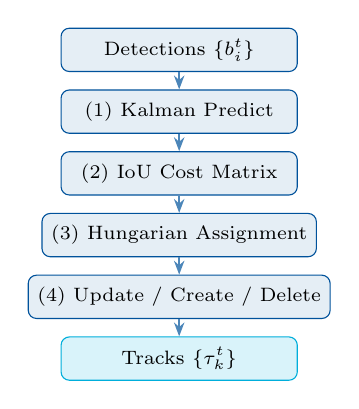
\begin{tikzpicture}[
            box/.style={draw=utecblue, fill=utecblue!10, rounded corners=3pt,
                minimum width=3.0cm, minimum height=0.55cm,
                font=\scriptsize, align=center},
            arr/.style={-{Stealth[length=5pt]}, utecblue!70, thick}
          ]
          \node[box] (det)  {Detections $\{b_i^t\}$};
          \node[box, below=0.22cm of det]  (pred) {(1) Kalman Predict};
          \node[box, below=0.22cm of pred] (iou)  {(2) IoU Cost Matrix};
          \node[box, below=0.22cm of iou]  (hung) {(3) Hungarian Assignment};
          \node[box, below=0.22cm of hung] (upd)  {(4) Update / Create / Delete};
          \node[box, below=0.22cm of upd, fill=uteccyan!15, draw=uteccyan]
          (out)  {Tracks $\{\tau_k^t\}$};
          \draw[arr] (det)  -- (pred);
          \draw[arr] (pred) -- (iou);
          \draw[arr] (iou)  -- (hung);
          \draw[arr] (hung) -- (upd);
          \draw[arr] (upd)  -- (out);
        \end{tikzpicture}%
      }
    \end{column}
  \end{columns}
\end{frame}

% ── SLIDE 14: SORT FILTRO DE KALMAN ────────────────────────────────────────────
\begin{frame}{SORT: Kalman Filter for Motion Prediction}
  \textbf{State vector} (7-dimensional, one Kalman filter per track):
  \[
    \mathbf{x} = \bigl[c_x,\; c_y,\; s,\; r,\; \dot{c}_x,\; \dot{c}_y,\; \dot{s}\bigr]^\top
  \]
  where $c_x, c_y$: bbox centre $\cdot$ $s = w \cdot h$: area $\cdot$
  $r = w/h$: aspect ratio (assumed constant) $\cdot$ $\dot{(\cdot)}$: velocity

  \begin{columns}[T]
    \begin{column}{0.48\textwidth}
      \textbf{Prediction step} (before observing detections):
      \[
        \mathbf{x}^-_t = F\,\mathbf{x}_{t-1}, \qquad
        P^-_t = F P_{t-1} F^\top + Q
      \]
      $F$: constant-velocity transition matrix \quad
      $P$: state covariance \quad $Q$: process noise
    \end{column}
    \begin{column}{0.48\textwidth}
      \textbf{Update step} (after associating a detection $\mathbf{z}=[c_x,c_y,s,r]^\top$):
      \[
        K = P^-_t H^\top\!\bigl(H P^-_t H^\top + R\bigr)^{-1}
      \]
      \[
        \mathbf{x}_t = \mathbf{x}^-_t + K\!\left(\mathbf{z} - H\mathbf{x}^-_t\right),
        \quad P_t = (I - KH)\,P^-_t
      \]
      $H$: observation matrix \quad $R$: measurement noise \quad
      $K$: Kalman gain (weights prediction vs.\ measurement)
    \end{column}
  \end{columns}
  \vspace{0.2em}
\end{frame}

% ── SLIDE 9: SORT HÚNGARO Y GESTIÓN ───────────────────────────────────────────
\begin{frame}{SORT: Hungarian Assignment and Track Lifecycle}
  \begin{columns}[T]
    \begin{column}{0.50\textwidth}
      \textbf{IoU-based cost matrix:}
      \[
        C_{ij} = 1 - \mathrm{IoU}(\hat{\tau}_i,\, b_j^t)
      \]
      where $\hat{\tau}_i$: Kalman-predicted bbox of track $i$,\;
      $b_j^t$: detection $j$ at time $t$

      \textbf{Hungarian algorithm} minimises total cost:
      \[
        \sigma^* = \arg\min_{\sigma} \sum_i C_{i,\sigma(i)}
      \]
      Match rejected if $\mathrm{IoU} < \tau_\mathrm{IoU} = 0.3$
      \vspace{0.3em}
      \begin{alertblock}{Separate trackers per class}
        \small Independent SORT instances for pedestrians and cars
        prevent cross-class identity confusion.
      \end{alertblock}
    \end{column}
    \begin{column}{0.46\textwidth}
      \textbf{Track lifecycle:}
      \vspace{0.2em}
      \resizebox{\linewidth}{!}{%
        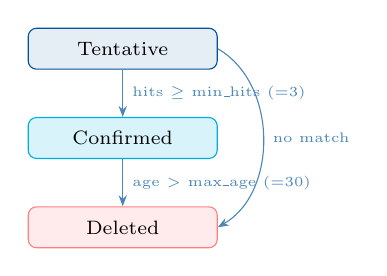
\begin{tikzpicture}[
            st/.style={draw=utecblue, rounded corners=3pt, fill=utecblue!10,
                minimum width=2.4cm, minimum height=0.52cm,
                font=\scriptsize, align=center},
            arr/.style={-{Stealth[length=4pt]}, utecblue!70}
          ]
          \node[st] (tent) {Tentative};
          \node[st, below=0.6cm of tent, fill=uteccyan!15, draw=uteccyan]
          (conf) {Confirmed};
          \node[st, below=0.6cm of conf, fill=red!8, draw=red!50]
          (dead) {Deleted};
          \draw[arr] (tent) -- node[right,font=\tiny]{hits $\geq$ min\_hits (=3)} (conf);
          \draw[arr] (conf) -- node[right,font=\tiny]{age $>$ max\_age (=30)} (dead);
          \draw[arr] (tent.east) to[bend left=60]
          node[right,font=\tiny]{no match} (dead.east);
        \end{tikzpicture}
      }
    \end{column}
  \end{columns}
\end{frame}

% ── SLIDE 10: PIPELINE COMPLETO ───────────────────────────────────────────────
\begin{frame}{Full Pipeline: YOLOv11 + SORT}
  \centering
  \vspace{-0.2cm}
  \resizebox{0.92\textwidth}{!}{%
    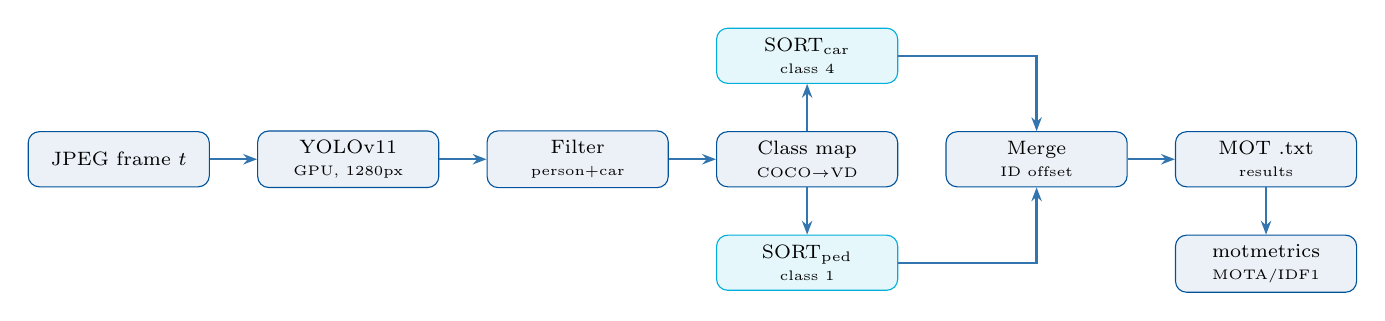
\begin{tikzpicture}[
        box/.style={draw=utecblue, fill=utecblue!8, rounded corners=4pt,
            minimum width=2.3cm, minimum height=0.7cm,
            font=\scriptsize, align=center},
        dbox/.style={draw=uteccyan, fill=uteccyan!10, rounded corners=4pt,
            minimum width=2.3cm, minimum height=0.7cm,
            font=\scriptsize, align=center},
        arr/.style={-{Stealth[length=5pt]}, utecblue!80, thick},
        note/.style={font=\tiny, text=utecblue!70, align=center}
      ]
      \node[box]  (fr)   {JPEG frame $t$};
      \node[box,  right=0.6cm of fr]  (yolo) {YOLOv11\\{\tiny GPU, 1280px}};
      \node[box,  right=0.6cm of yolo](filt) {Filter\\{\tiny person+car}};
      \node[box,  right=0.6cm of filt](map)  {Class map\\{\tiny COCO$\to$VD}};
      \node[dbox, below=0.6cm of map] (sp)   {SORT\textsubscript{ped}\\{\tiny class 1}};
      \node[dbox, above=0.6cm of map] (sc)   {SORT\textsubscript{car}\\{\tiny class 4}};
      \node[box,  right=0.6cm of map] (merge){Merge\\{\tiny ID offset}};
      \node[box,  right=0.6cm of merge](mot) {MOT .txt\\{\tiny results}};
      \node[box,  below=0.6cm of mot] (eval) {motmetrics\\{\tiny MOTA/IDF1}};

      \draw[arr] (fr)   -- (yolo);
      \draw[arr] (yolo) -- (filt);
      \draw[arr] (filt) -- (map);
      \draw[arr] (map.south) -- (sp.north);
      \draw[arr] (map.north) -- (sc.south);
      \draw[arr] (sp.east)   -| (merge.south);
      \draw[arr] (sc.east)   -| (merge.north);
      \draw[arr] (merge) -- (mot);
      \draw[arr] (mot.south) -- (eval.north);
    \end{tikzpicture}
  }

  \vspace{0.4em}
  \begin{columns}[T]
    \begin{column}{0.48\textwidth}
      \begin{block}{Key design choice}
        \small Separate SORT trackers per class.
        Car IDs offset by $+100\,000$ to prevent
        ID collision across classes in the output file.
      \end{block}
    \end{column}
    \begin{column}{0.48\textwidth}
      \begin{block}{Output format (MOT standard)}
        \scriptsize
        \texttt{frame, id, x, y, w, h, conf, class, vis}\\
        One line per detection per frame.
        Sorted by \texttt{(frame, id)}.
      \end{block}
    \end{column}
  \end{columns}
\end{frame}

% ── SLIDE 15: DEMO ÉXITO FRAMES ───────────────────────────────────────────────
\begin{frame}{Qualitative Demo --- Success Case (Track Continuity)}
  \begin{columns}[T]
    \begin{column}{0.32\textwidth}
      \centering
      {\small\textbf{Frame $t$}}\\[3pt]
      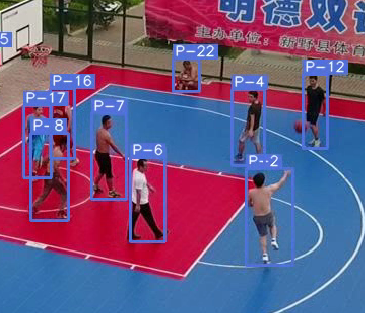
\includegraphics[width=\linewidth]{figures/yolo11_success_f1.png}
    \end{column}
    \begin{column}{0.32\textwidth}
      \centering
      {\small\textbf{Frame $t+15$}}\\[3pt]
      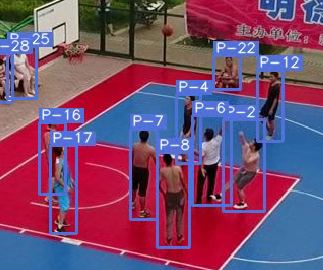
\includegraphics[width=\linewidth]{figures/yolo11_success_f2.png}
    \end{column}
    \begin{column}{0.32\textwidth}
      \centering
      {\small\textbf{Frame $t+30$}}\\[3pt]
      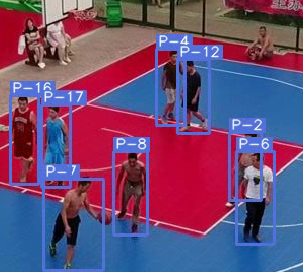
\includegraphics[width=\linewidth]{figures/yolo11_success_f3.png}
    \end{column}
  \end{columns}
  \vspace{0.4em}
  \begin{block}{Look!}
    \small Same coloured bounding boxes and numeric IDs across the three
    frames, demonstrating that SORT maintains identity through motion.
  \end{block}
\end{frame}

% ── SLIDE 17: DEMO FALLO FRAMES ───────────────────────────────────────────────
\begin{frame}{Qualitative Demo --- Failure Case (ID Switch)}
  \begin{columns}[T]
    \begin{column}{0.32\textwidth}
      \centering
      {\small\textbf{Before occlusion}}\\[3pt]
      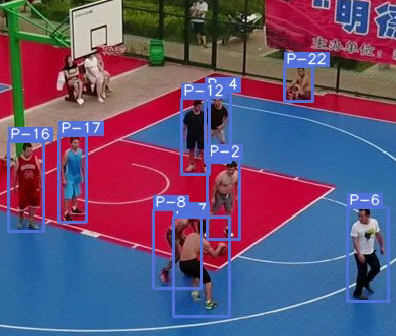
\includegraphics[width=\linewidth]{figures/yolo11_fail_f1.png}
    \end{column}
    \begin{column}{0.32\textwidth}
      \centering
      {\small\textbf{During occlusion}}\\[3pt]
      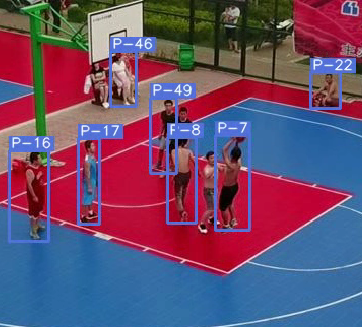
\includegraphics[width=\linewidth]{figures/yolo11_fail_f2.png}
    \end{column}
    \begin{column}{0.32\textwidth}
      \centering
      {\small\textbf{After occlusion}}\\[3pt]
      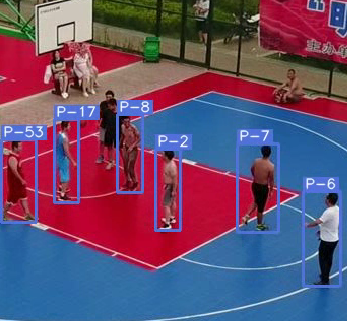
\includegraphics[width=\linewidth]{figures/yolo11_fail_f3.png}
    \end{column}
  \end{columns}
  \vspace{0.4em}
  \begin{block}{ID Switch}
    \small When an object is occluded for $>\!$ \texttt{max\_age} frames,
    SORT deletes the track. On reappearance, no Kalman prediction
    is available $\Rightarrow$ a new ID is assigned.
  \end{block}
\end{frame}

% ── SLIDE 19: REFERENCIAS ─────────────────────────────────────────────────────
\begin{frame}[allowframebreaks]{References}
  \footnotesize
  \begin{thebibliography}{9}

    \bibitem{zhu2022visdrone}
    P.~Zhu, L.~Wen, D.~Du, X.~Bian, H.~Fan, Q.~Hu, and H.~Ling,
    ``Detection and Tracking Meet Drones Challenge,''
    \textit{IEEE Transactions on Pattern Analysis and Machine Intelligence},
    vol.~44, no.~11, pp.~7380--7399, Nov.~2022.
    DOI: 10.1109/TPAMI.2021.3119563.

    \bibitem{bewley2016sort}
    A.~Bewley, Z.~Ge, L.~Ott, F.~Ramos, and B.~Upcroft,
    ``Simple Online and Realtime Tracking,''
    in \textit{Proc. IEEE Int. Conf. Image Processing (ICIP)},
    Phoenix, AZ, Sep.~2016, pp.~3464--3468.
    DOI: 10.1109/ICIP.2016.7533003.

    \bibitem{lin2014coco}
    T.-Y.~Lin, M.~Maire, S.~Belongie, J.~Hays, P.~Perona, D.~Ramanan,
    P.~Dollár, and C.~L.~Zitnick,
    ``Microsoft COCO: Common Objects in Context,''
    in \textit{Proc. European Conf. Computer Vision (ECCV)},
    Zurich, Switzerland, Sep.~2014, pp.~740--755.
    DOI: 10.1007/978-3-319-10602-1\_48.

    \bibitem{ultralytics2024yolo11}
    Ultralytics,
    ``YOLOv11: A Leap Forward in Real-Time Object Detection,''
    \textit{Ultralytics Documentation}, 2024.
      [Online]. Available: \url{https://docs.ultralytics.com/models/yolo11/}

    \bibitem{kalman1960}
    R.~E.~Kalman,
    ``A New Approach to Linear Filtering and Prediction Problems,''
    \textit{Journal of Basic Engineering},
    vol.~82, no.~1, pp.~35--45, Mar.~1960.
    DOI: 10.1115/1.3662552.

    \bibitem{kuhn1955hungarian}
    H.~W.~Kuhn,
    ``The Hungarian Method for the Assignment Problem,''
    \textit{Naval Research Logistics Quarterly},
    vol.~2, no.~1--2, pp.~83--97, 1955.
    DOI: 10.1002/nav.3800020109.

    \bibitem{wojke2017deepsort}
    N.~Wojke, A.~Bewley, and D.~Paulus,
    ``Simple Online and Realtime Tracking with a Deep Association Metric,''
    in \textit{Proc. IEEE Int. Conf. Image Processing (ICIP)},
    Beijing, China, Sep.~2017, pp.~3645--3649.
    DOI: 10.1109/ICIP.2017.8296962.

    \bibitem{aharon2022botsort}
    N.~Aharon, R.~Orfaig, and B.-Z.~Bobrovsky,
    ``BoT-SORT: Robust Associations Multi-Pedestrian Tracking,''
    \textit{arXiv preprint arXiv:2206.14651}, Jun.~2022.
      [Online]. Available: \url{https://arxiv.org/abs/2206.14651}

    \bibitem{akbari2022sahi}
    O.~F.~Cengiz, F.~Akyon, E.~Altinuc, and A.~Tekin,
    ``Slicing Aided Hyper Inference and Fine-tuning for
    Small Object Detection,''
    in \textit{Proc. IEEE Int. Conf. Image Processing (ICIP)},
    Bordeaux, France, Oct.~2022, pp.~966--970.
    DOI: 10.1109/ICIP46576.2022.9897990.

  \end{thebibliography}
\end{frame}

% ── SLIDE 20: CIERRE ──────────────────────────────────────────────────────────
{
  \setbeamercolor{background canvas}{bg=utecblue}
  \begin{frame}[plain]
    \centering
    \vspace{2cm}
    {\color{white}\Huge\bfseries Thank you\par}
    \vspace{0.8em}
    {\color{uteccyan}\large Questions?\par}
    \vspace{1.5em}
    {\color{white!70}Computer Vision --- UTEC, 2026-I\par}
    \vspace{0.3em}
    {\color{white!50}\small Assignment IV: Detection and Tracking --- Method 1 Baseline\par}
  \end{frame}
}

\end{document}
